\documentclass[11pt]{article}
\usepackage[textwidth=18.0cm, textheight=23.0cm, top=2.0cm]{geometry}
\usepackage{pst-all}
\usepackage{amssymb}
\usepackage{tikz}
\usepackage{underscore}\begin{document}
\pagestyle{empty}


ClassName: \underline{\textbf{Class_08.2bp-23}}
\par
BinSize: \underline{\textbf{100 × 100}}
\par
ReduceSize: \underline{\textbf{100 × 100}}
\par
TypeNum: \underline{\textbf{60}}
\par
Num: \underline{\textbf{60}}
\par
OutS: \underline{\textbf{150000}}
\par
InS: \underline{\textbf{124539}}
\par
Rate: \underline{\textbf{0.830}}
\par
UB: \underline{\textbf{15}}
\par
LB0: \underline{\textbf{15}}
\par
LB: \underline{\textbf{15}}
\par
LBWithCut: \underline{\textbf{15}}
\par
NodeCut: \underline{\textbf{0}}
\par
ExtendedNodeCnt: \underline{\textbf{1}}
\par
GenNodeCnt: \underline{\textbf{1}}
\par
PrimalNode: \underline{\textbf{0}}
\par
ColumnCount: \underline{\textbf{15}}
\par
TotalCutCount: \underline{\textbf{0}}
\par
RootCutCount: \underline{\textbf{0}}
\par
LPSolverCnt: \underline{\textbf{1}}
\par
PricingSolverCnt: \underline{\textbf{0}}
\par
BranchAndBoundNum: \underline{\textbf{1}}
\par
isOpt: \underline{\textbf{true}}
\par
TimeOnInitSolution: \underline{\textbf{0.170 s}}
\par
TimeOnPrimal: \underline{\textbf{0.000 s}}
\par
TimeOnPricing: \underline{\textbf{0.000 s}}
\par
TimeOnRmp: \underline{\textbf{0.063 s}}
\par
TotalTime: \underline{\textbf{0.295 s}}
\par
\newpage


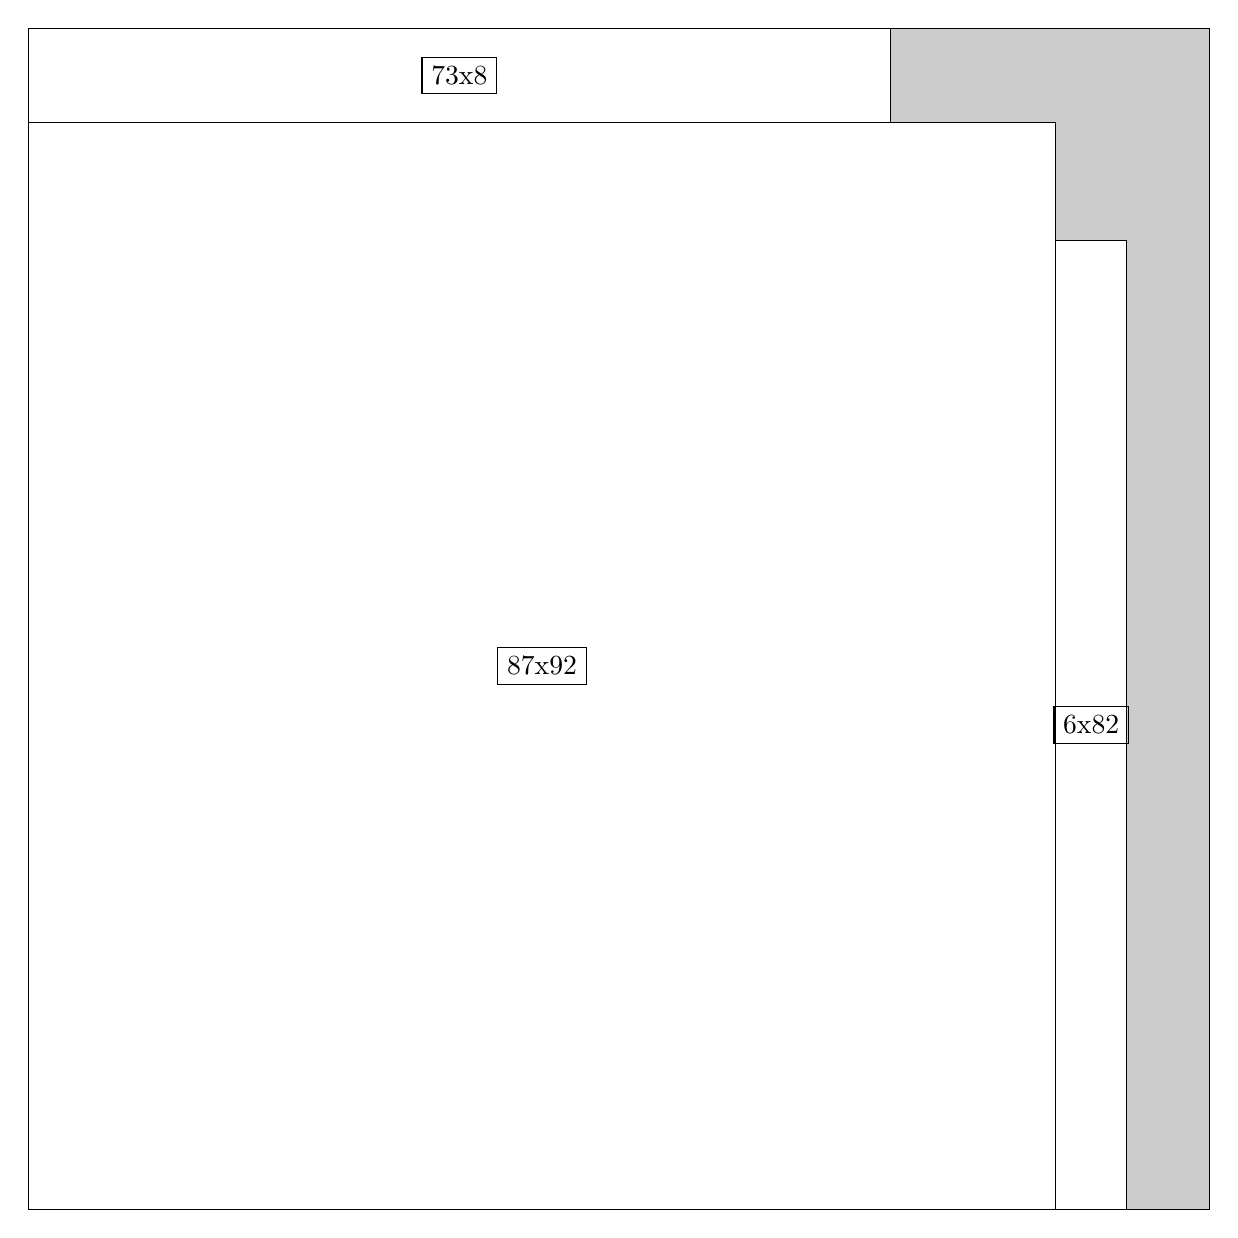
\begin{tikzpicture}[shorten >=1pt,scale=1.0,every node/.style={scale=1.0},->]
\tikzstyle{vertex}=[circle,fill=black!25,minimum size=14pt,inner sep=0pt]
\filldraw[fill=gray!40!white, draw=black] (0,0) rectangle (15.0,15.0);
\foreach \name/\x/\y/\w/\h in {87x92/0.0/0.0/13.049999999999999/13.799999999999999,73x8/0.0/13.799999999999999/10.95/1.2,6x82/13.049999999999999/0.0/0.8999999999999999/12.299999999999999}
\filldraw[fill=white!40!white, draw=black] (\x,\y) rectangle node[draw] (\name) {\name} ++(\w,\h);
\end{tikzpicture}


w =87 , h =92 , x =0 , y =0 , v =8004
\par
w =73 , h =8 , x =0 , y =92 , v =584
\par
w =6 , h =82 , x =87 , y =0 , v =492
\par
\newpage


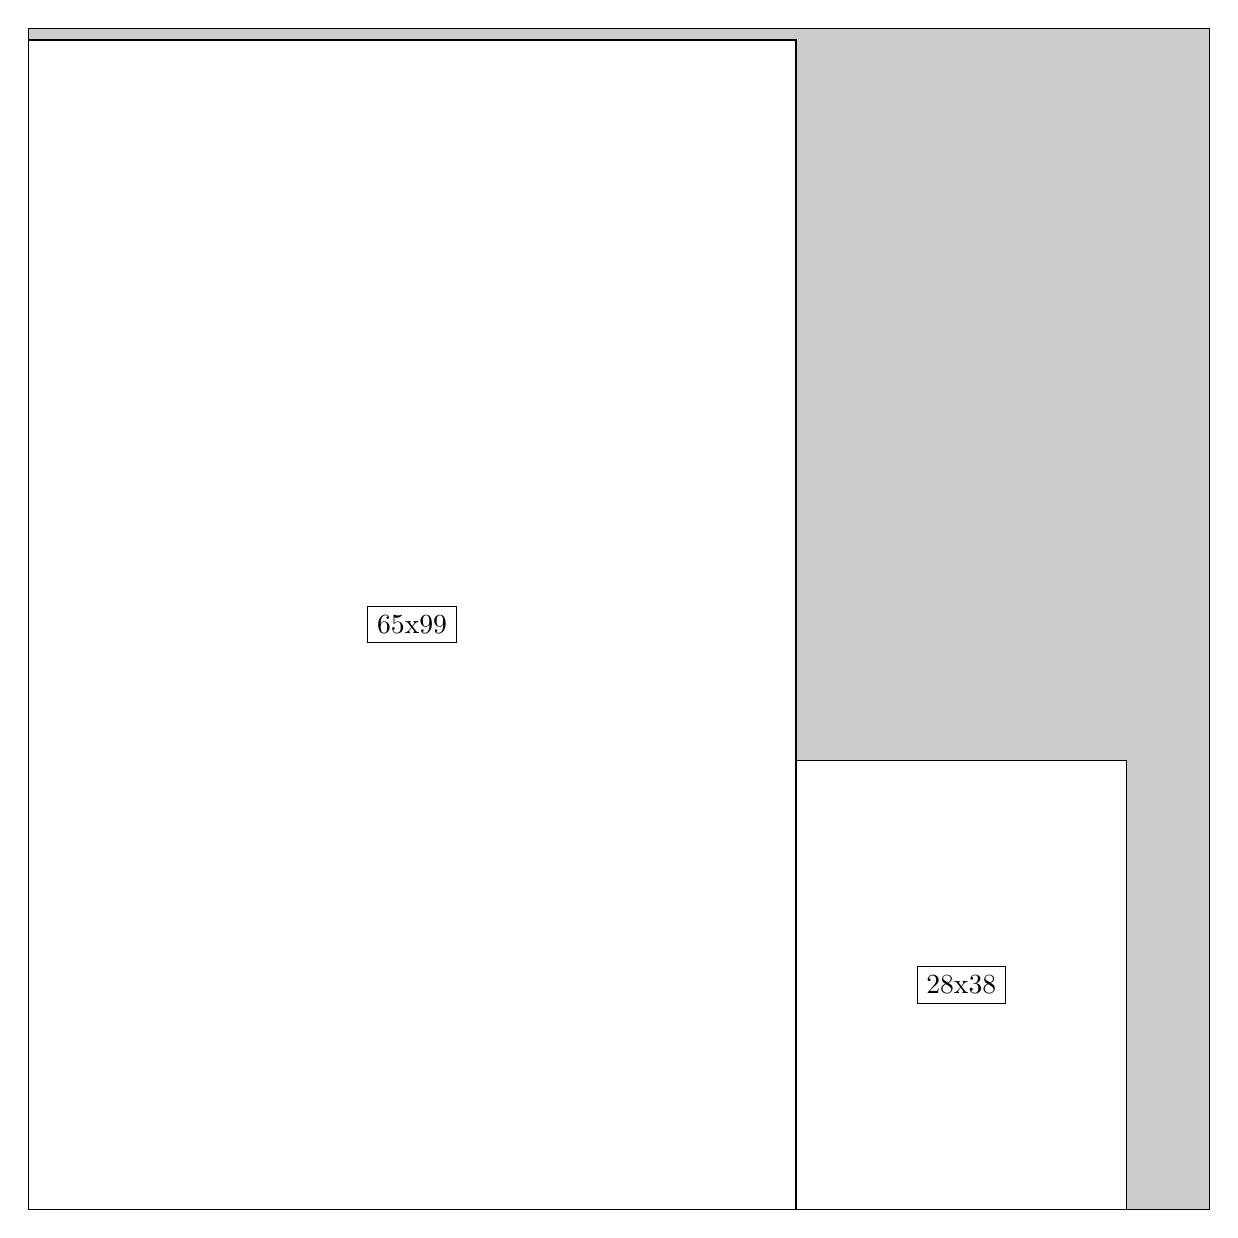
\begin{tikzpicture}[shorten >=1pt,scale=1.0,every node/.style={scale=1.0},->]
\tikzstyle{vertex}=[circle,fill=black!25,minimum size=14pt,inner sep=0pt]
\filldraw[fill=gray!40!white, draw=black] (0,0) rectangle (15.0,15.0);
\foreach \name/\x/\y/\w/\h in {65x99/0.0/0.0/9.75/14.85,28x38/9.75/0.0/4.2/5.7}
\filldraw[fill=white!40!white, draw=black] (\x,\y) rectangle node[draw] (\name) {\name} ++(\w,\h);
\end{tikzpicture}


w =65 , h =99 , x =0 , y =0 , v =6435
\par
w =28 , h =38 , x =65 , y =0 , v =1064
\par
\newpage


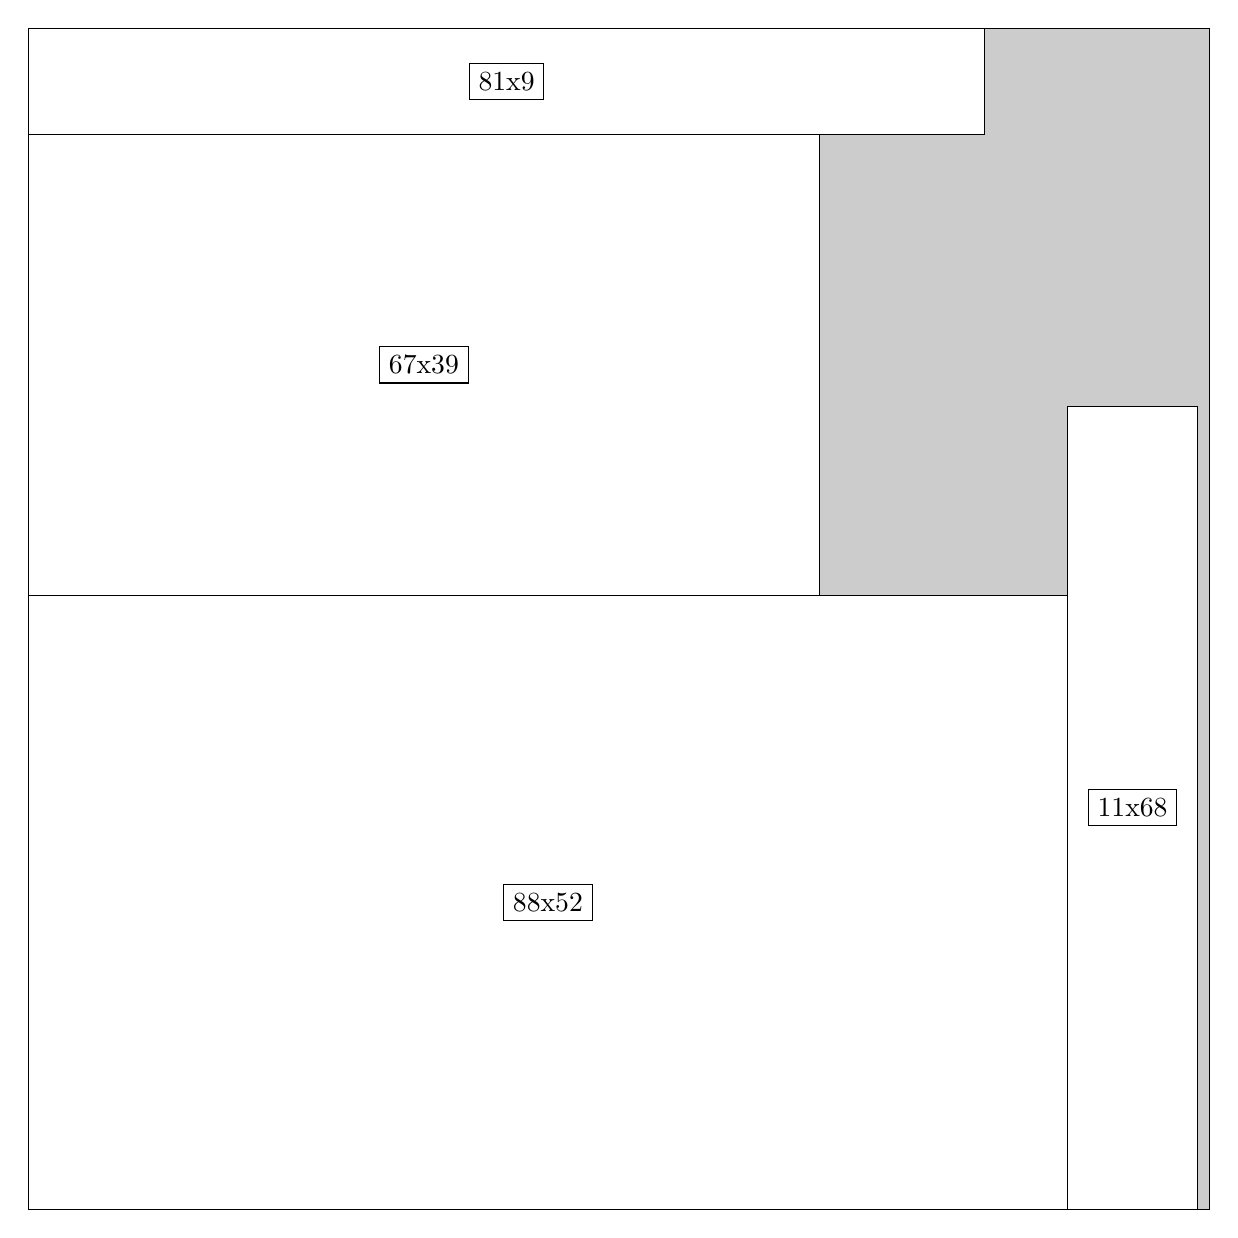
\begin{tikzpicture}[shorten >=1pt,scale=1.0,every node/.style={scale=1.0},->]
\tikzstyle{vertex}=[circle,fill=black!25,minimum size=14pt,inner sep=0pt]
\filldraw[fill=gray!40!white, draw=black] (0,0) rectangle (15.0,15.0);
\foreach \name/\x/\y/\w/\h in {88x52/0.0/0.0/13.2/7.8,67x39/0.0/7.8/10.049999999999999/5.85,11x68/13.2/0.0/1.65/10.2,81x9/0.0/13.65/12.15/1.3499999999999999}
\filldraw[fill=white!40!white, draw=black] (\x,\y) rectangle node[draw] (\name) {\name} ++(\w,\h);
\end{tikzpicture}


w =88 , h =52 , x =0 , y =0 , v =4576
\par
w =67 , h =39 , x =0 , y =52 , v =2613
\par
w =11 , h =68 , x =88 , y =0 , v =748
\par
w =81 , h =9 , x =0 , y =91 , v =729
\par
\newpage


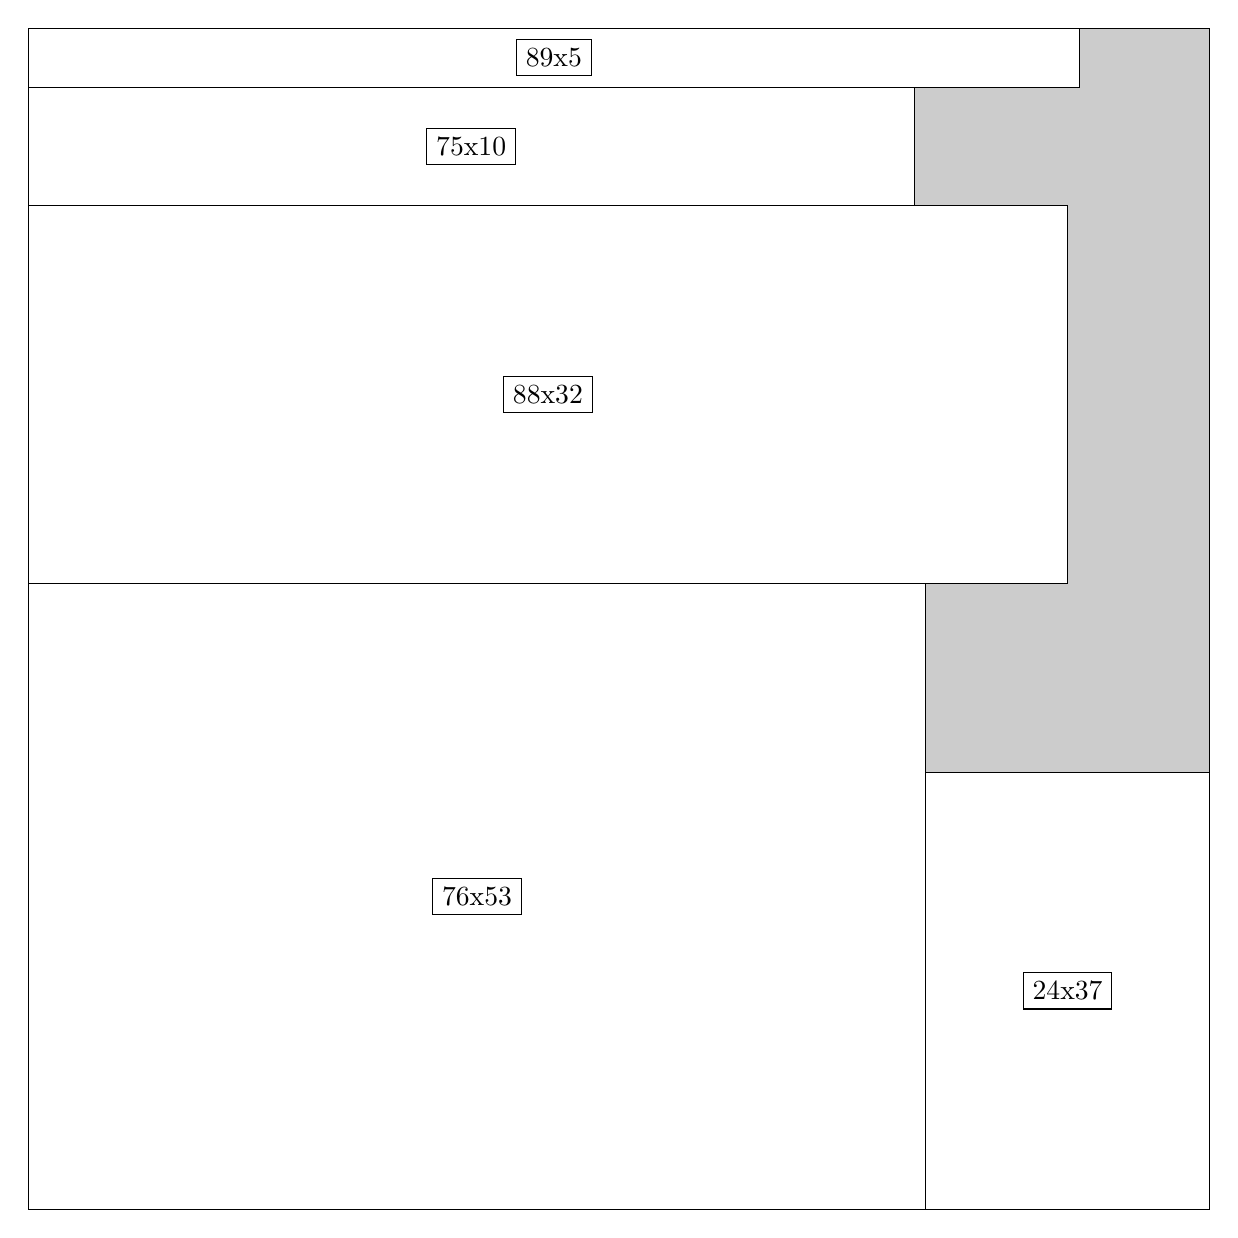
\begin{tikzpicture}[shorten >=1pt,scale=1.0,every node/.style={scale=1.0},->]
\tikzstyle{vertex}=[circle,fill=black!25,minimum size=14pt,inner sep=0pt]
\filldraw[fill=gray!40!white, draw=black] (0,0) rectangle (15.0,15.0);
\foreach \name/\x/\y/\w/\h in {76x53/0.0/0.0/11.4/7.949999999999999,88x32/0.0/7.949999999999999/13.2/4.8,24x37/11.4/0.0/3.5999999999999996/5.55,75x10/0.0/12.75/11.25/1.5,89x5/0.0/14.25/13.35/0.75}
\filldraw[fill=white!40!white, draw=black] (\x,\y) rectangle node[draw] (\name) {\name} ++(\w,\h);
\end{tikzpicture}


w =76 , h =53 , x =0 , y =0 , v =4028
\par
w =88 , h =32 , x =0 , y =53 , v =2816
\par
w =24 , h =37 , x =76 , y =0 , v =888
\par
w =75 , h =10 , x =0 , y =85 , v =750
\par
w =89 , h =5 , x =0 , y =95 , v =445
\par
\newpage


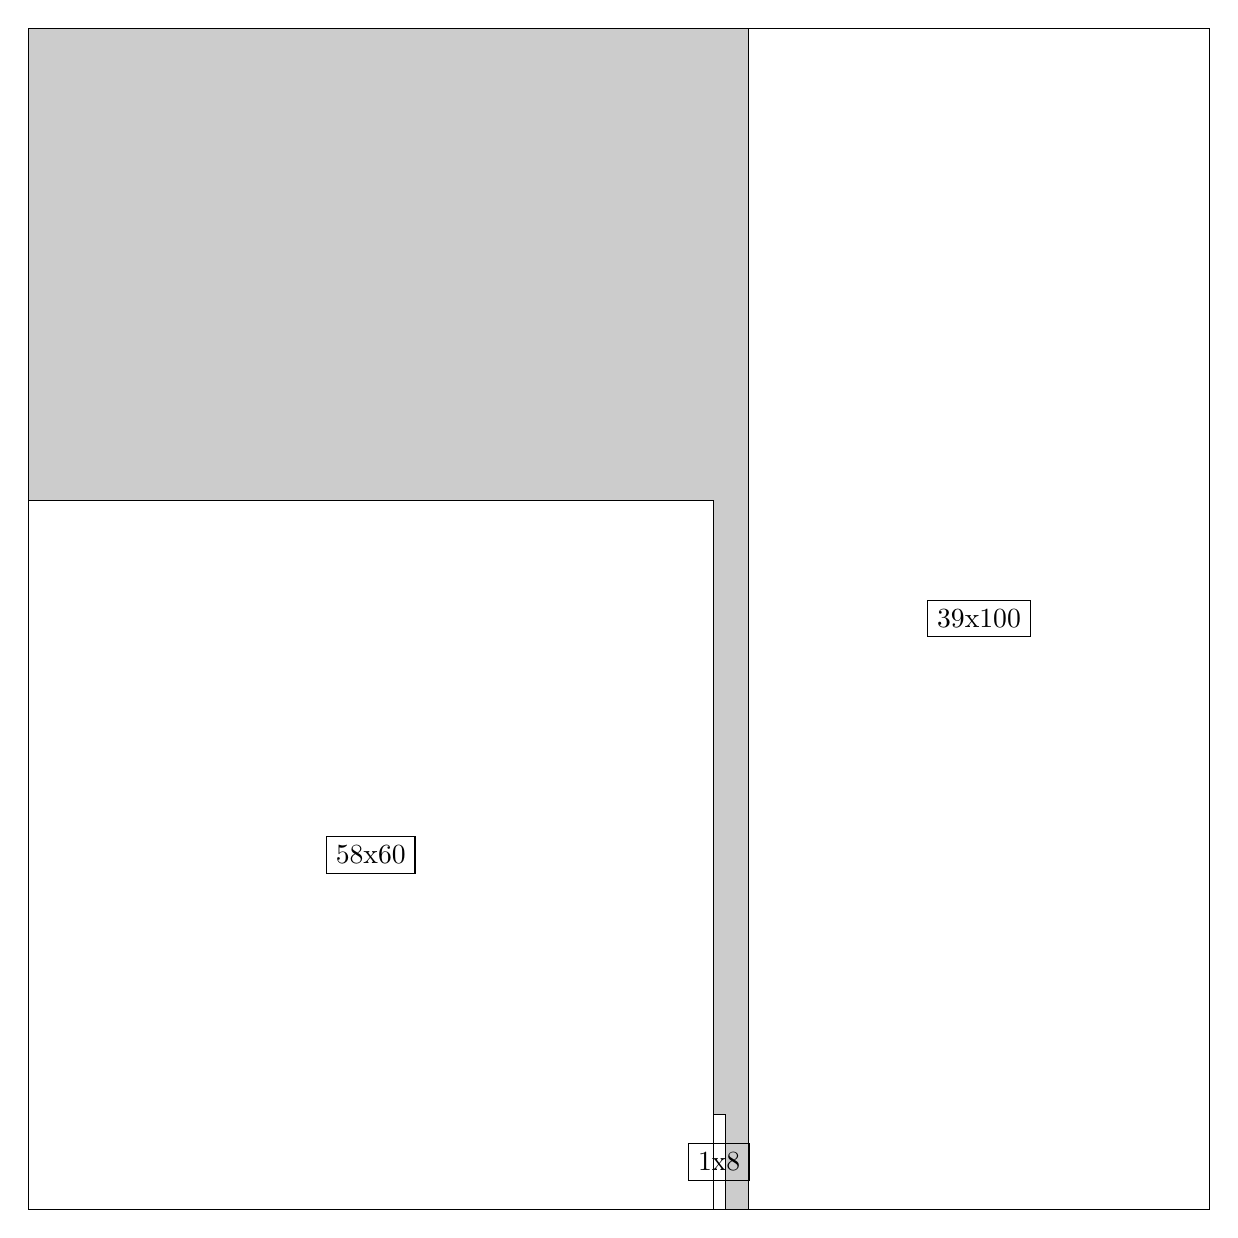
\begin{tikzpicture}[shorten >=1pt,scale=1.0,every node/.style={scale=1.0},->]
\tikzstyle{vertex}=[circle,fill=black!25,minimum size=14pt,inner sep=0pt]
\filldraw[fill=gray!40!white, draw=black] (0,0) rectangle (15.0,15.0);
\foreach \name/\x/\y/\w/\h in {39x100/9.15/0.0/5.85/15.0,58x60/0.0/0.0/8.7/9.0,1x8/8.7/0.0/0.15/1.2}
\filldraw[fill=white!40!white, draw=black] (\x,\y) rectangle node[draw] (\name) {\name} ++(\w,\h);
\end{tikzpicture}


w =39 , h =100 , x =61 , y =0 , v =3900
\par
w =58 , h =60 , x =0 , y =0 , v =3480
\par
w =1 , h =8 , x =58 , y =0 , v =8
\par
\newpage


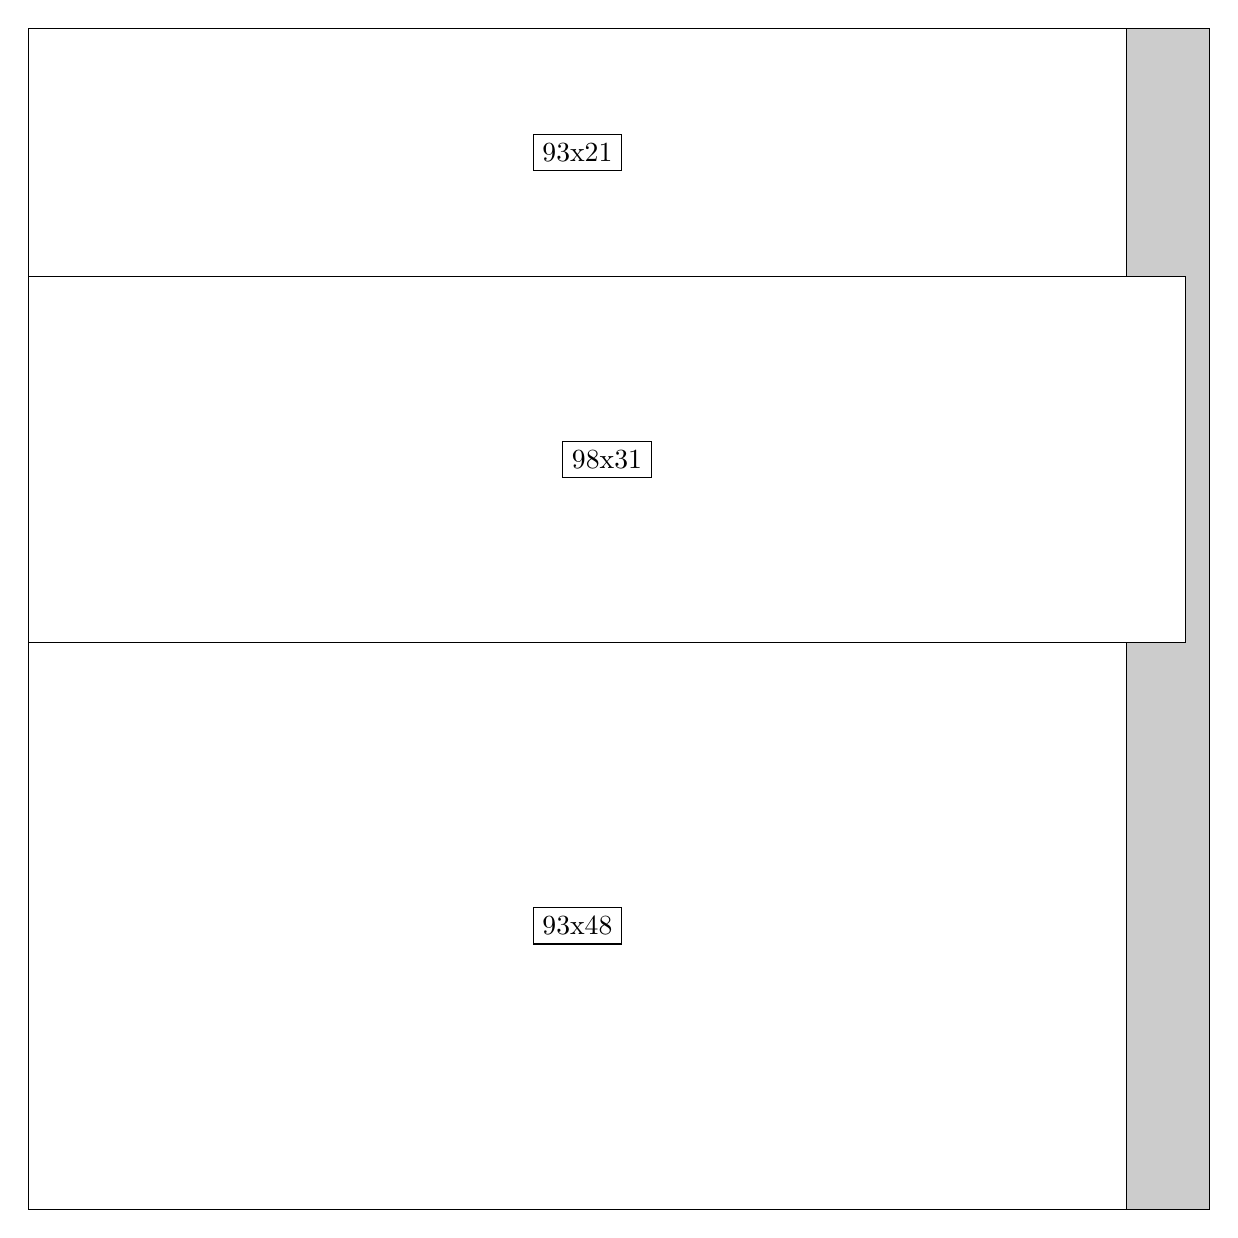
\begin{tikzpicture}[shorten >=1pt,scale=1.0,every node/.style={scale=1.0},->]
\tikzstyle{vertex}=[circle,fill=black!25,minimum size=14pt,inner sep=0pt]
\filldraw[fill=gray!40!white, draw=black] (0,0) rectangle (15.0,15.0);
\foreach \name/\x/\y/\w/\h in {93x48/0.0/0.0/13.95/7.199999999999999,98x31/0.0/7.199999999999999/14.7/4.6499999999999995,93x21/0.0/11.85/13.95/3.15}
\filldraw[fill=white!40!white, draw=black] (\x,\y) rectangle node[draw] (\name) {\name} ++(\w,\h);
\end{tikzpicture}


w =93 , h =48 , x =0 , y =0 , v =4464
\par
w =98 , h =31 , x =0 , y =48 , v =3038
\par
w =93 , h =21 , x =0 , y =79 , v =1953
\par
\newpage


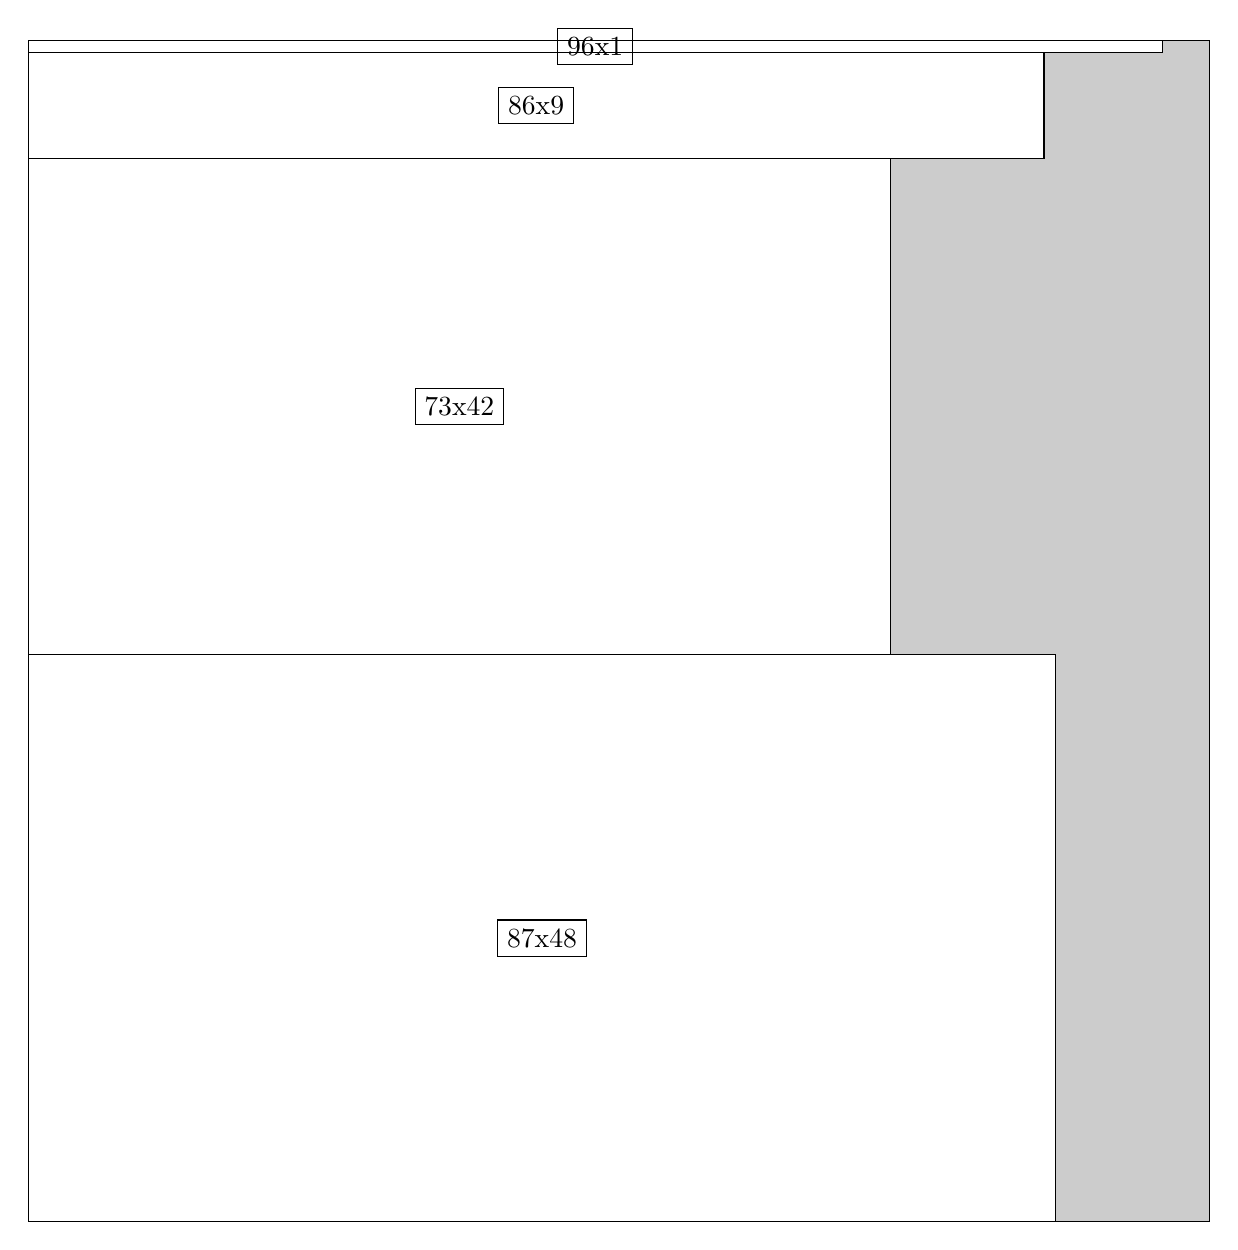
\begin{tikzpicture}[shorten >=1pt,scale=1.0,every node/.style={scale=1.0},->]
\tikzstyle{vertex}=[circle,fill=black!25,minimum size=14pt,inner sep=0pt]
\filldraw[fill=gray!40!white, draw=black] (0,0) rectangle (15.0,15.0);
\foreach \name/\x/\y/\w/\h in {87x48/0.0/0.0/13.049999999999999/7.199999999999999,73x42/0.0/7.199999999999999/10.95/6.3,86x9/0.0/13.5/12.9/1.3499999999999999,96x1/0.0/14.85/14.399999999999999/0.15}
\filldraw[fill=white!40!white, draw=black] (\x,\y) rectangle node[draw] (\name) {\name} ++(\w,\h);
\end{tikzpicture}


w =87 , h =48 , x =0 , y =0 , v =4176
\par
w =73 , h =42 , x =0 , y =48 , v =3066
\par
w =86 , h =9 , x =0 , y =90 , v =774
\par
w =96 , h =1 , x =0 , y =99 , v =96
\par
\newpage


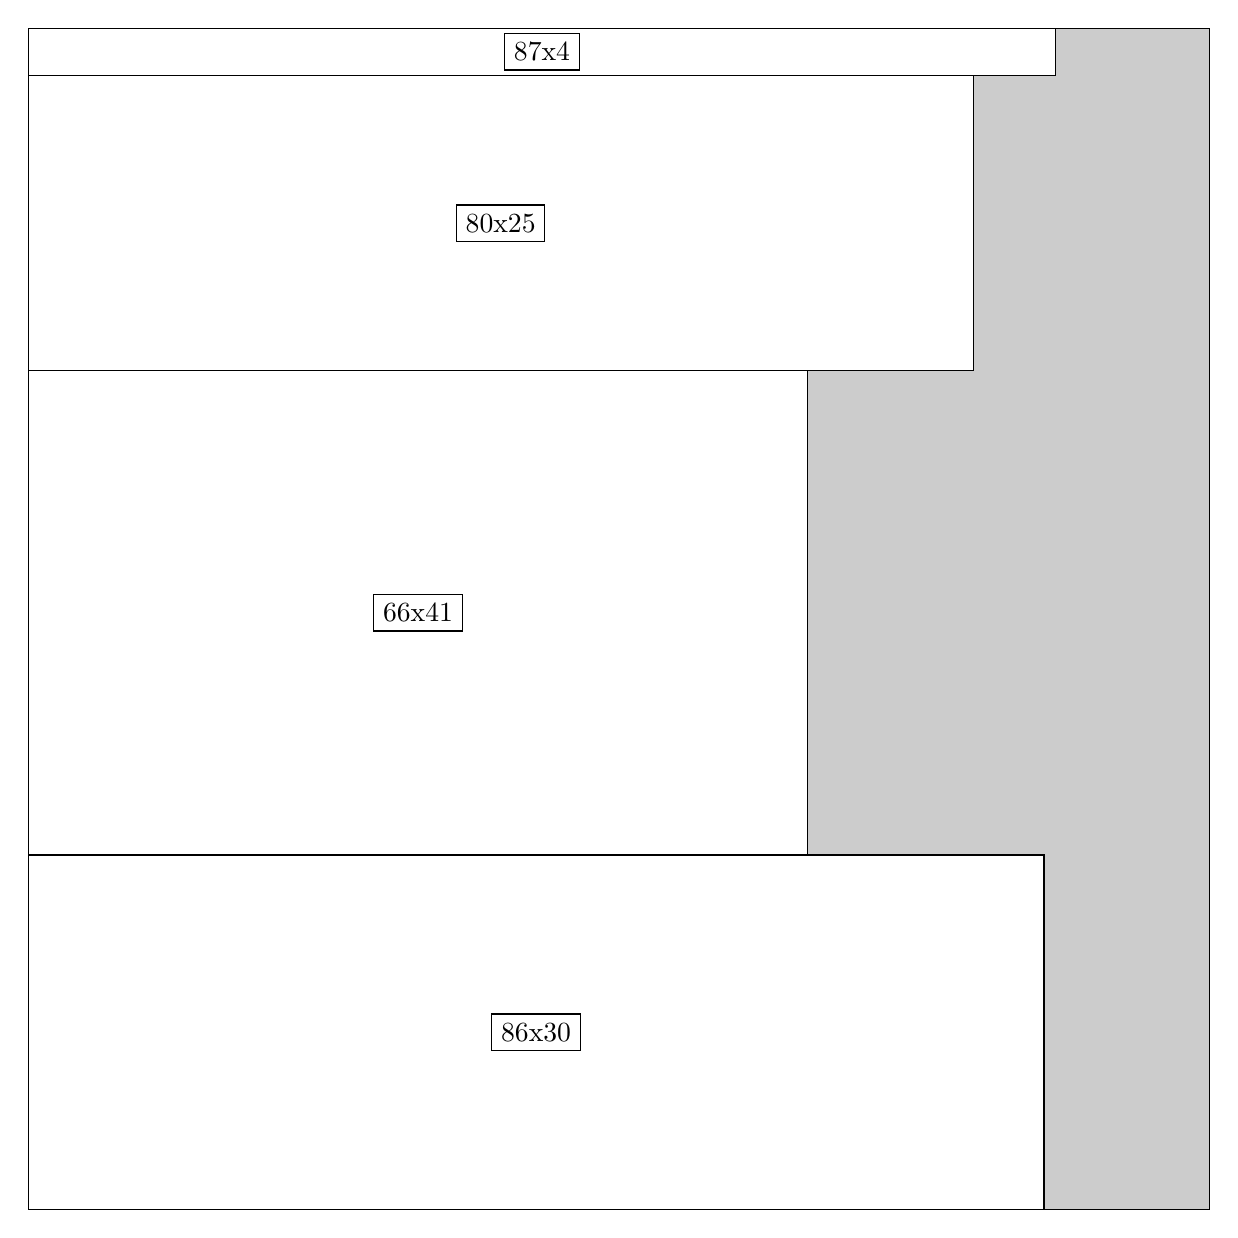
\begin{tikzpicture}[shorten >=1pt,scale=1.0,every node/.style={scale=1.0},->]
\tikzstyle{vertex}=[circle,fill=black!25,minimum size=14pt,inner sep=0pt]
\filldraw[fill=gray!40!white, draw=black] (0,0) rectangle (15.0,15.0);
\foreach \name/\x/\y/\w/\h in {86x30/0.0/0.0/12.9/4.5,66x41/0.0/4.5/9.9/6.1499999999999995,80x25/0.0/10.65/12.0/3.75,87x4/0.0/14.399999999999999/13.049999999999999/0.6}
\filldraw[fill=white!40!white, draw=black] (\x,\y) rectangle node[draw] (\name) {\name} ++(\w,\h);
\end{tikzpicture}


w =86 , h =30 , x =0 , y =0 , v =2580
\par
w =66 , h =41 , x =0 , y =30 , v =2706
\par
w =80 , h =25 , x =0 , y =71 , v =2000
\par
w =87 , h =4 , x =0 , y =96 , v =348
\par
\newpage


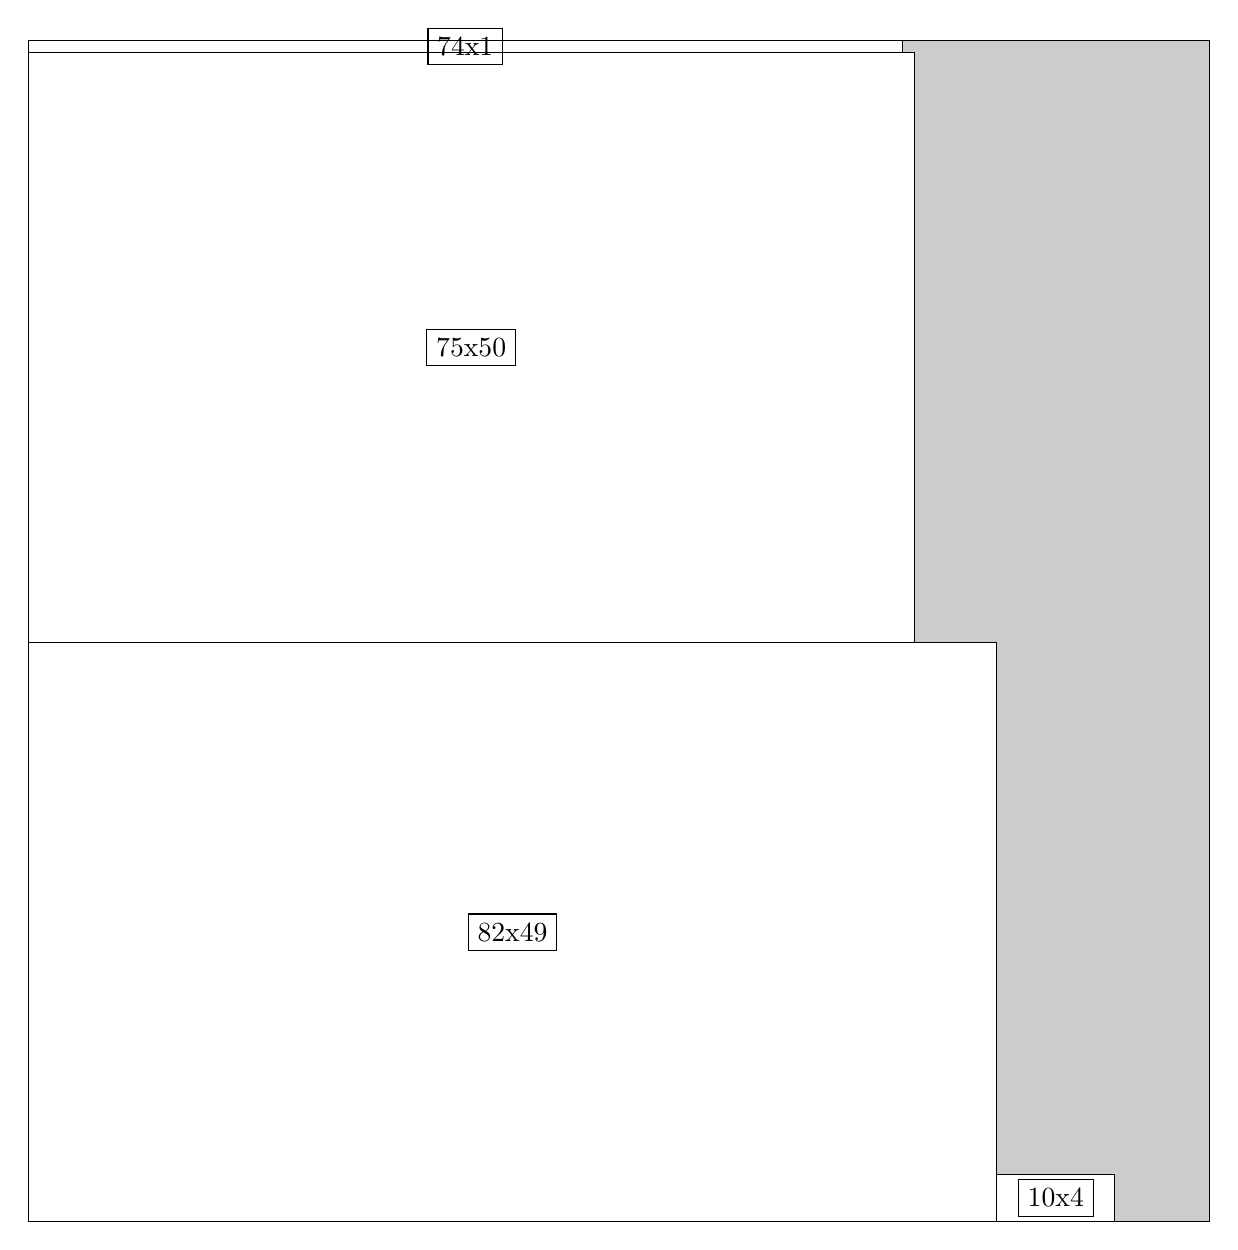
\begin{tikzpicture}[shorten >=1pt,scale=1.0,every node/.style={scale=1.0},->]
\tikzstyle{vertex}=[circle,fill=black!25,minimum size=14pt,inner sep=0pt]
\filldraw[fill=gray!40!white, draw=black] (0,0) rectangle (15.0,15.0);
\foreach \name/\x/\y/\w/\h in {82x49/0.0/0.0/12.299999999999999/7.35,75x50/0.0/7.35/11.25/7.5,74x1/0.0/14.85/11.1/0.15,10x4/12.299999999999999/0.0/1.5/0.6}
\filldraw[fill=white!40!white, draw=black] (\x,\y) rectangle node[draw] (\name) {\name} ++(\w,\h);
\end{tikzpicture}


w =82 , h =49 , x =0 , y =0 , v =4018
\par
w =75 , h =50 , x =0 , y =49 , v =3750
\par
w =74 , h =1 , x =0 , y =99 , v =74
\par
w =10 , h =4 , x =82 , y =0 , v =40
\par
\newpage


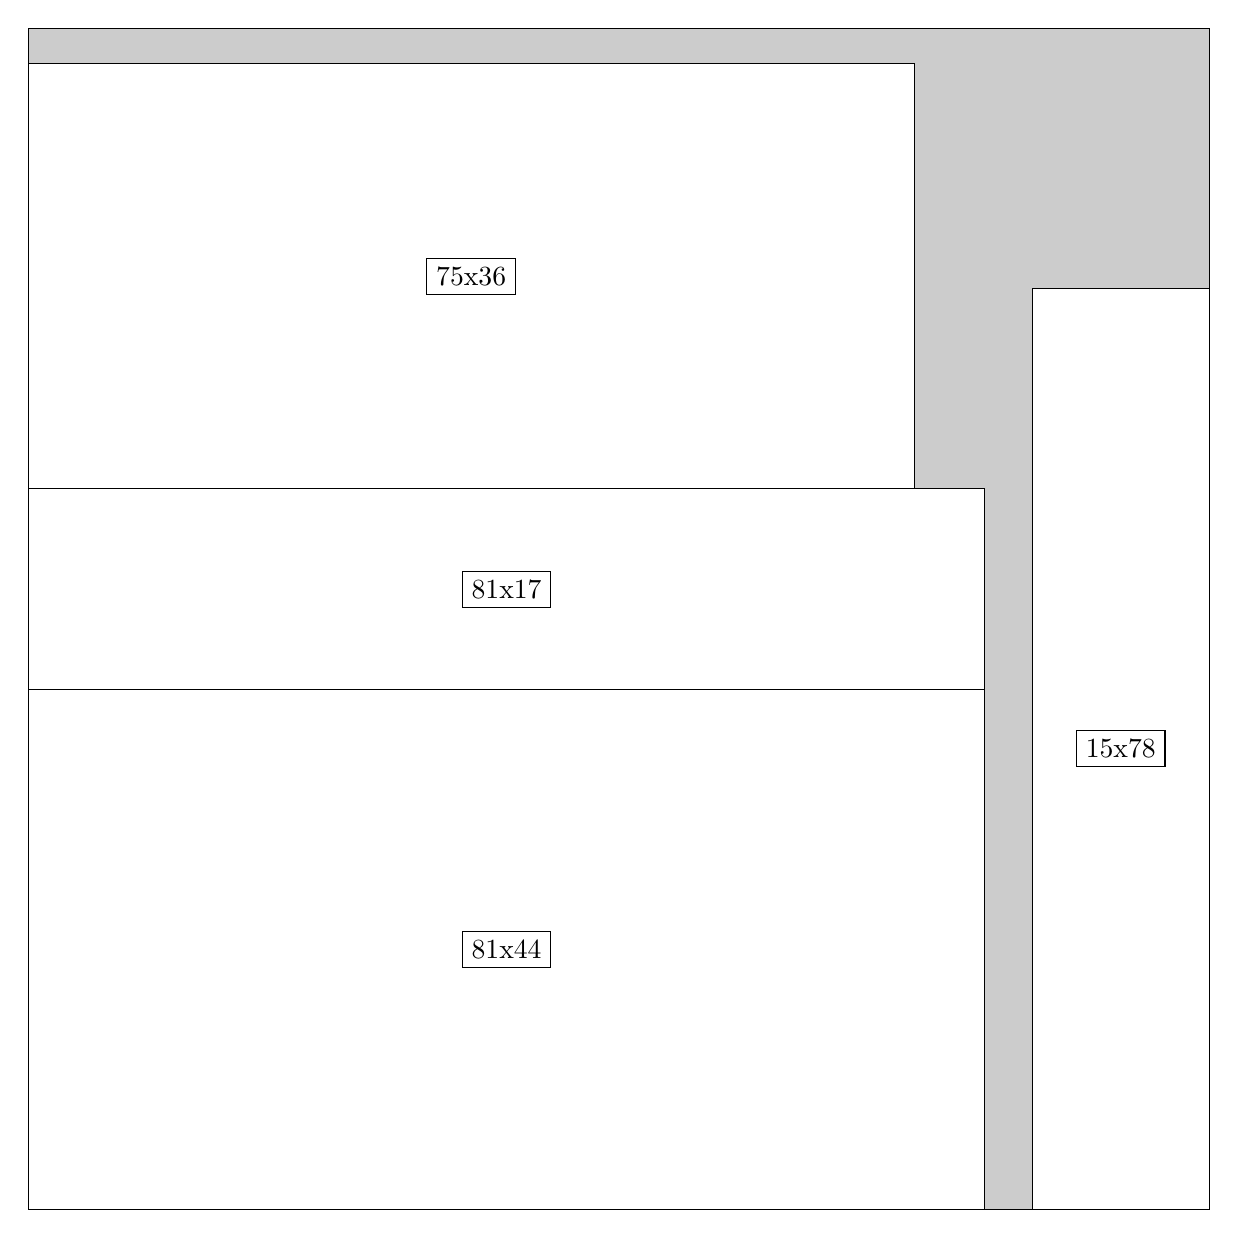
\begin{tikzpicture}[shorten >=1pt,scale=1.0,every node/.style={scale=1.0},->]
\tikzstyle{vertex}=[circle,fill=black!25,minimum size=14pt,inner sep=0pt]
\filldraw[fill=gray!40!white, draw=black] (0,0) rectangle (15.0,15.0);
\foreach \name/\x/\y/\w/\h in {81x44/0.0/0.0/12.15/6.6,75x36/0.0/9.15/11.25/5.3999999999999995,81x17/0.0/6.6/12.15/2.55,15x78/12.75/0.0/2.25/11.7}
\filldraw[fill=white!40!white, draw=black] (\x,\y) rectangle node[draw] (\name) {\name} ++(\w,\h);
\end{tikzpicture}


w =81 , h =44 , x =0 , y =0 , v =3564
\par
w =75 , h =36 , x =0 , y =61 , v =2700
\par
w =81 , h =17 , x =0 , y =44 , v =1377
\par
w =15 , h =78 , x =85 , y =0 , v =1170
\par
\newpage


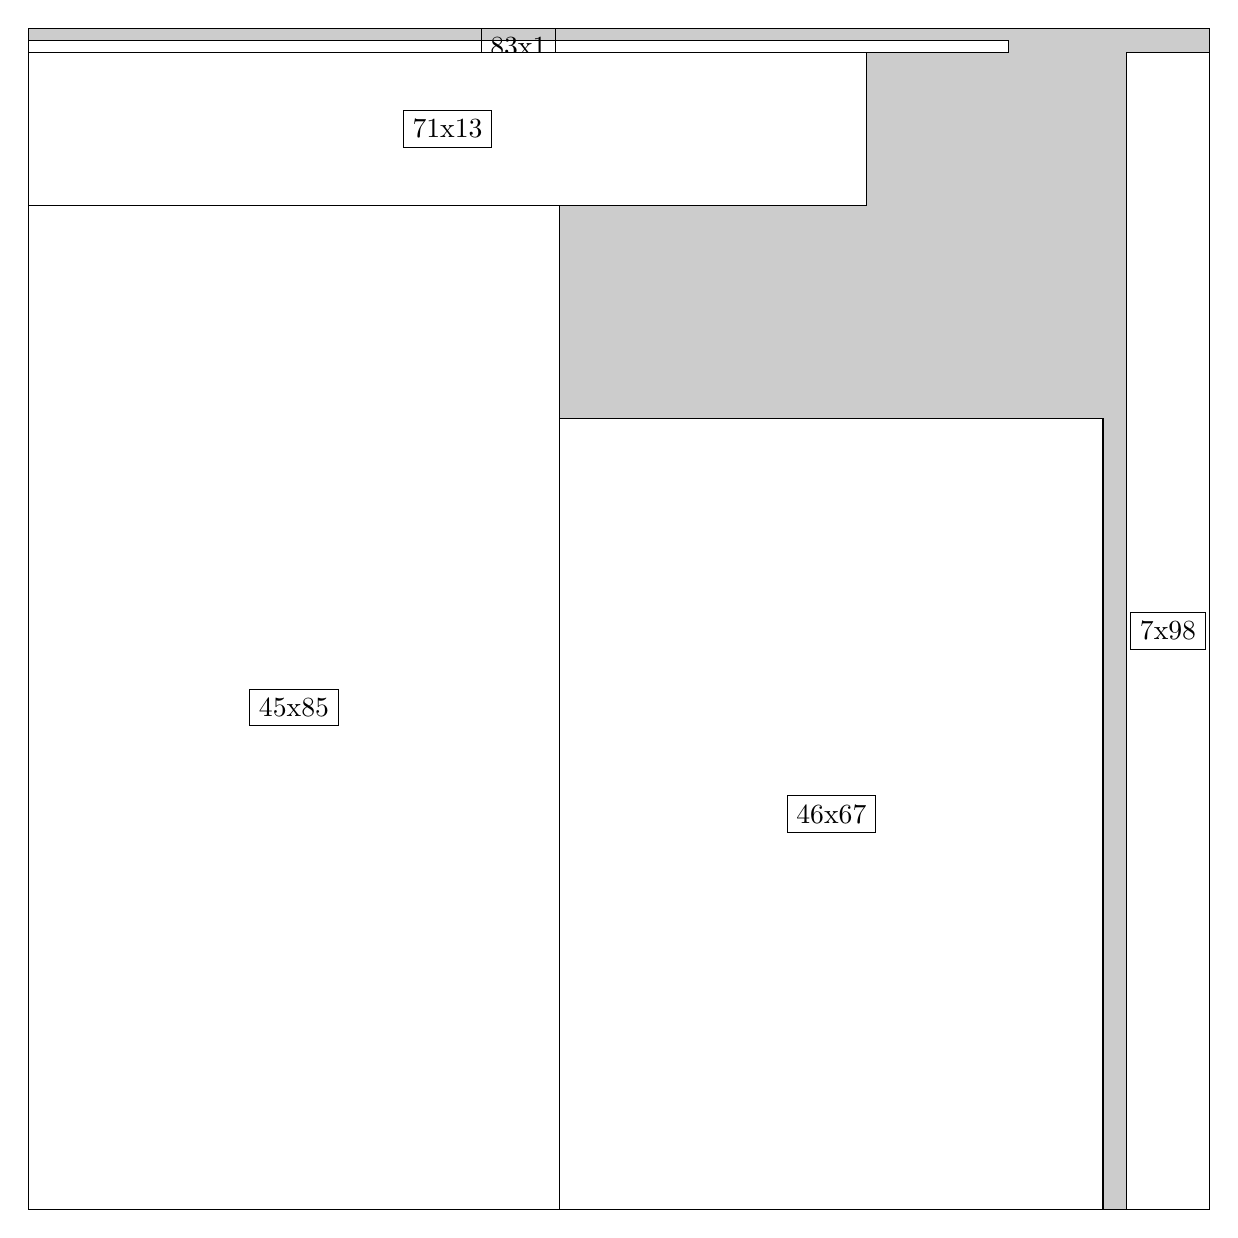
\begin{tikzpicture}[shorten >=1pt,scale=1.0,every node/.style={scale=1.0},->]
\tikzstyle{vertex}=[circle,fill=black!25,minimum size=14pt,inner sep=0pt]
\filldraw[fill=gray!40!white, draw=black] (0,0) rectangle (15.0,15.0);
\foreach \name/\x/\y/\w/\h in {45x85/0.0/0.0/6.75/12.75,46x67/6.75/0.0/6.8999999999999995/10.049999999999999,83x1/0.0/14.7/12.45/0.15,7x98/13.95/0.0/1.05/14.7,71x13/0.0/12.75/10.65/1.95}
\filldraw[fill=white!40!white, draw=black] (\x,\y) rectangle node[draw] (\name) {\name} ++(\w,\h);
\end{tikzpicture}


w =45 , h =85 , x =0 , y =0 , v =3825
\par
w =46 , h =67 , x =45 , y =0 , v =3082
\par
w =83 , h =1 , x =0 , y =98 , v =83
\par
w =7 , h =98 , x =93 , y =0 , v =686
\par
w =71 , h =13 , x =0 , y =85 , v =923
\par
\newpage


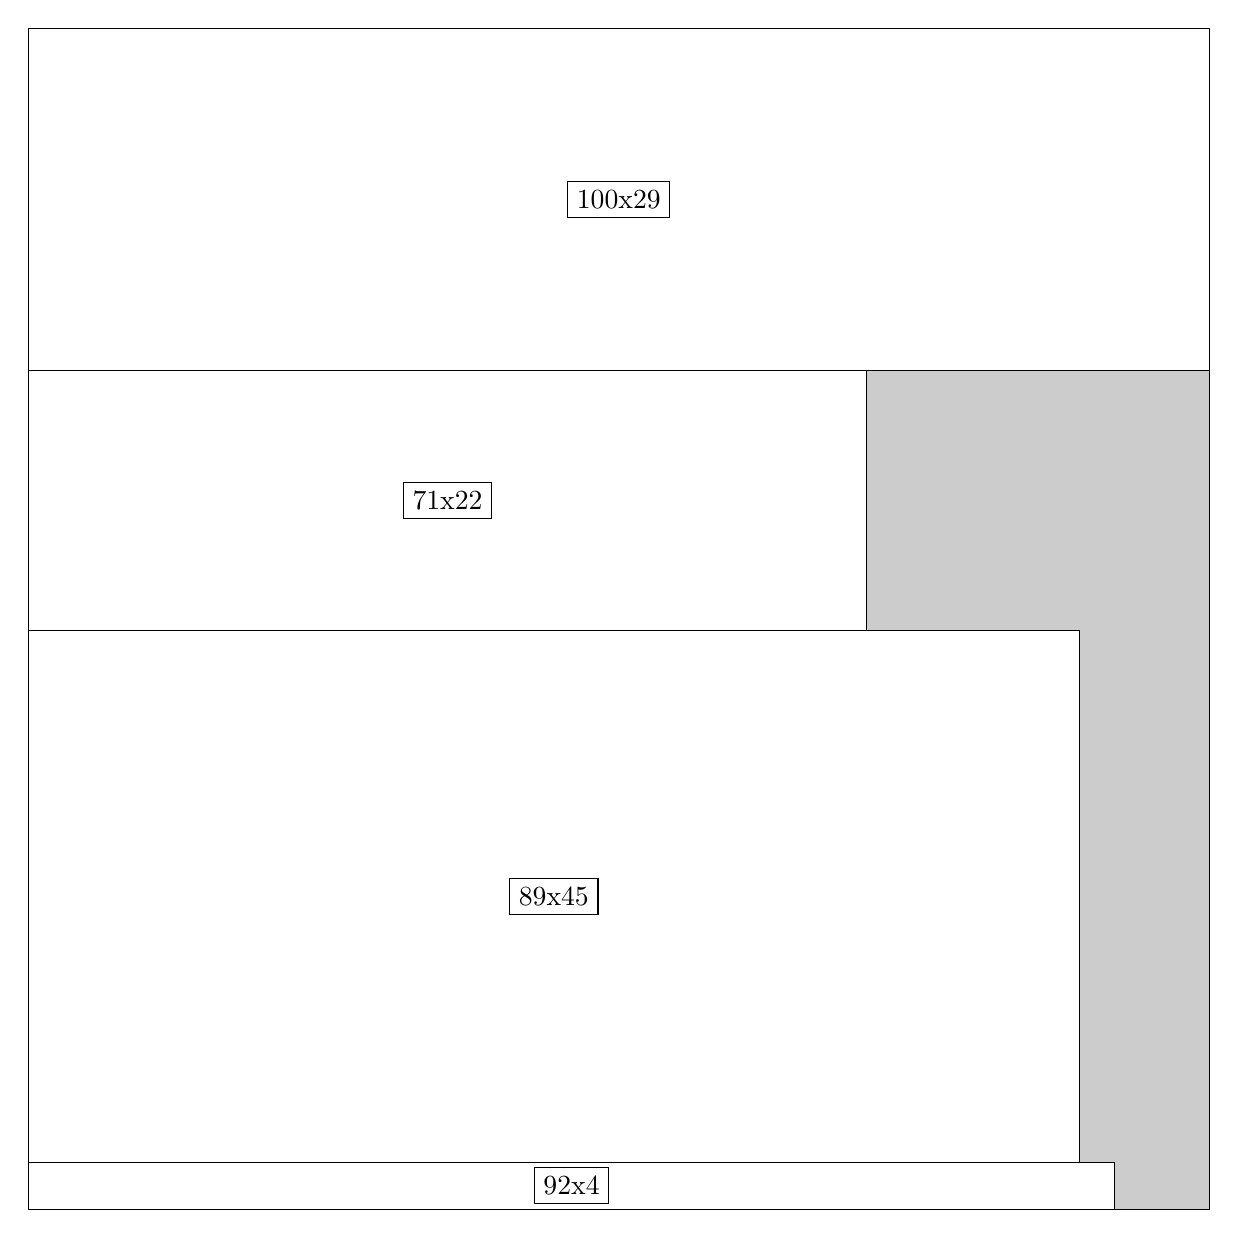
\begin{tikzpicture}[shorten >=1pt,scale=1.0,every node/.style={scale=1.0},->]
\tikzstyle{vertex}=[circle,fill=black!25,minimum size=14pt,inner sep=0pt]
\filldraw[fill=gray!40!white, draw=black] (0,0) rectangle (15.0,15.0);
\foreach \name/\x/\y/\w/\h in {89x45/0.0/0.6/13.35/6.75,100x29/0.0/10.65/15.0/4.35,71x22/0.0/7.35/10.65/3.3,92x4/0.0/0.0/13.799999999999999/0.6}
\filldraw[fill=white!40!white, draw=black] (\x,\y) rectangle node[draw] (\name) {\name} ++(\w,\h);
\end{tikzpicture}


w =89 , h =45 , x =0 , y =4 , v =4005
\par
w =100 , h =29 , x =0 , y =71 , v =2900
\par
w =71 , h =22 , x =0 , y =49 , v =1562
\par
w =92 , h =4 , x =0 , y =0 , v =368
\par
\newpage


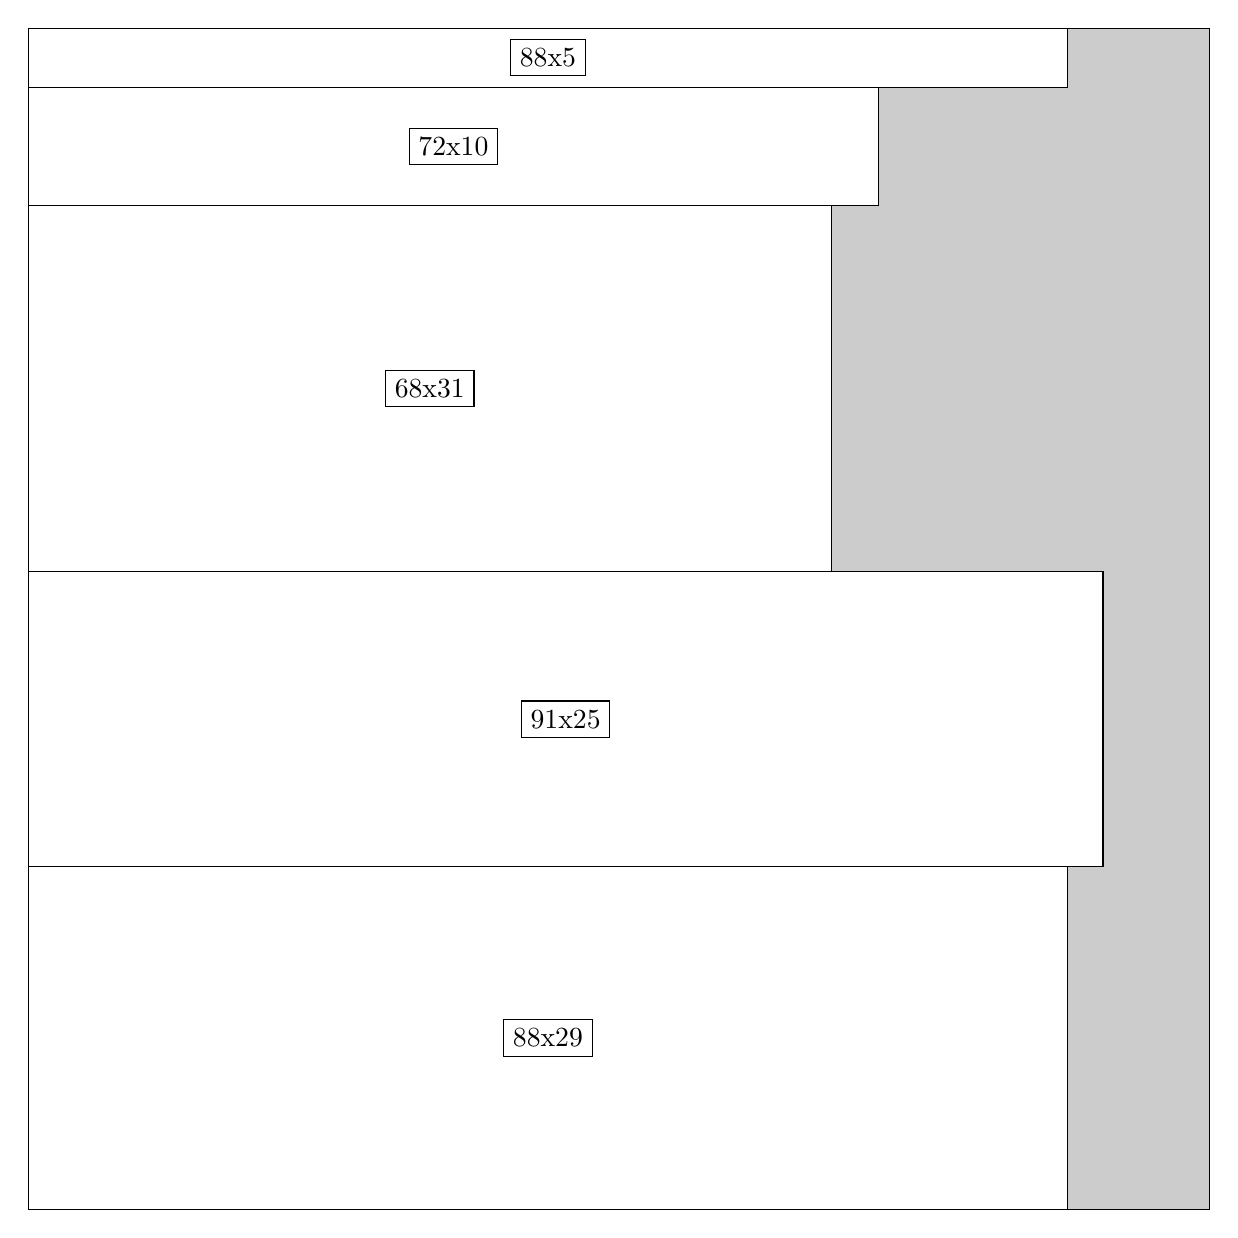
\begin{tikzpicture}[shorten >=1pt,scale=1.0,every node/.style={scale=1.0},->]
\tikzstyle{vertex}=[circle,fill=black!25,minimum size=14pt,inner sep=0pt]
\filldraw[fill=gray!40!white, draw=black] (0,0) rectangle (15.0,15.0);
\foreach \name/\x/\y/\w/\h in {88x29/0.0/0.0/13.2/4.35,91x25/0.0/4.35/13.65/3.75,68x31/0.0/8.1/10.2/4.6499999999999995,72x10/0.0/12.75/10.799999999999999/1.5,88x5/0.0/14.25/13.2/0.75}
\filldraw[fill=white!40!white, draw=black] (\x,\y) rectangle node[draw] (\name) {\name} ++(\w,\h);
\end{tikzpicture}


w =88 , h =29 , x =0 , y =0 , v =2552
\par
w =91 , h =25 , x =0 , y =29 , v =2275
\par
w =68 , h =31 , x =0 , y =54 , v =2108
\par
w =72 , h =10 , x =0 , y =85 , v =720
\par
w =88 , h =5 , x =0 , y =95 , v =440
\par
\newpage


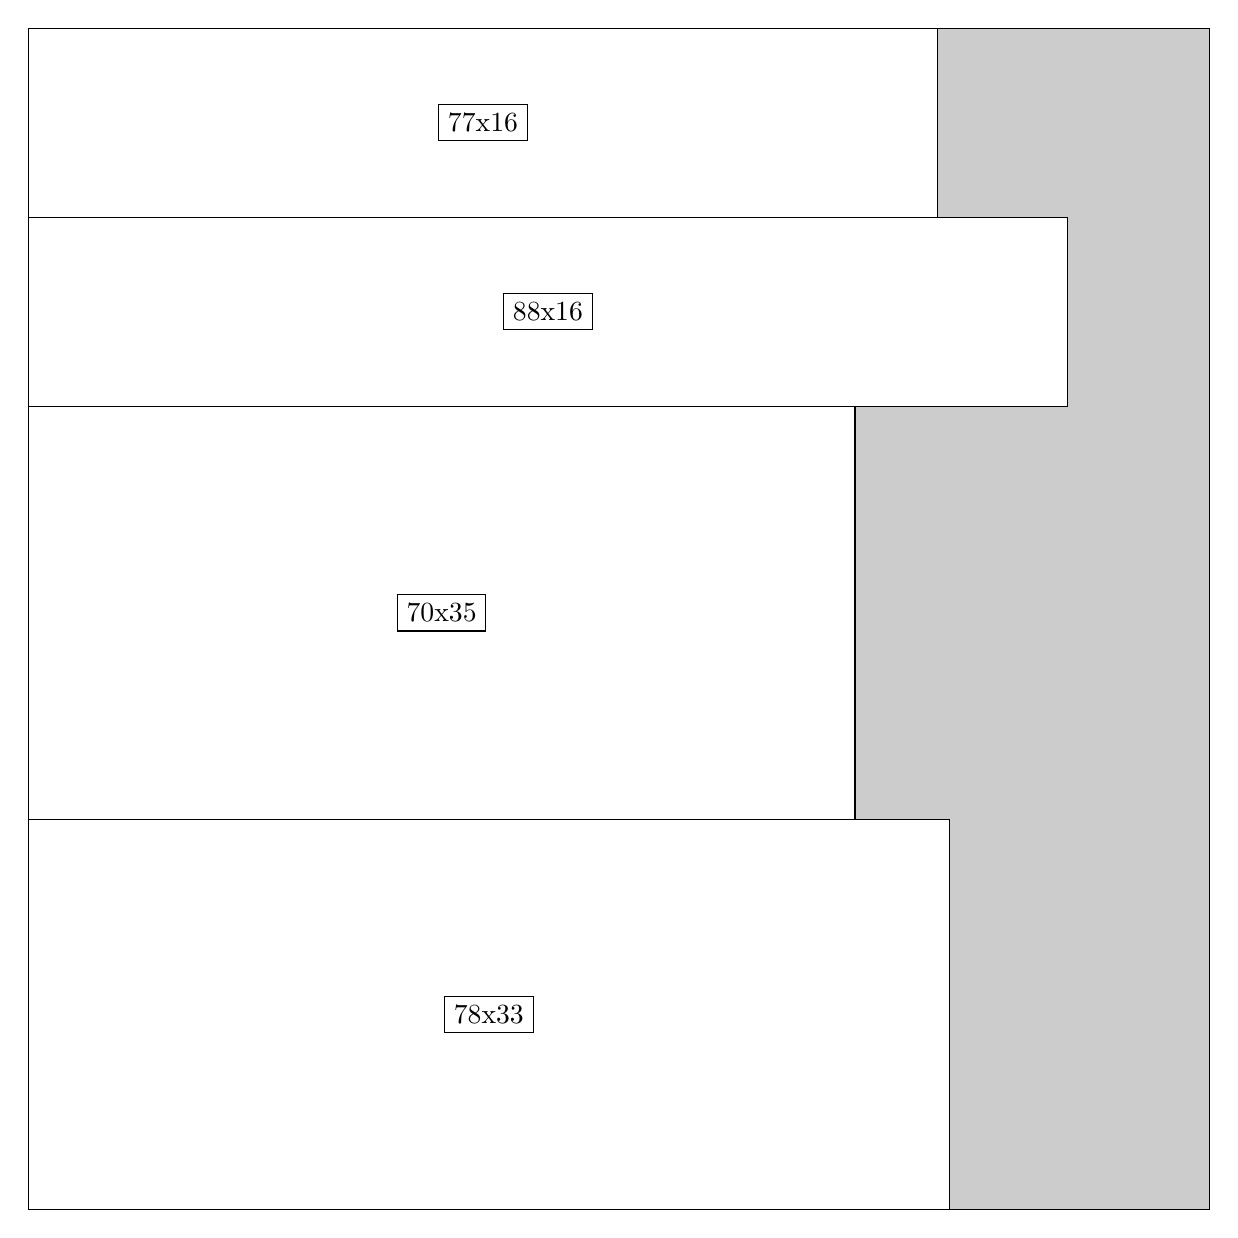
\begin{tikzpicture}[shorten >=1pt,scale=1.0,every node/.style={scale=1.0},->]
\tikzstyle{vertex}=[circle,fill=black!25,minimum size=14pt,inner sep=0pt]
\filldraw[fill=gray!40!white, draw=black] (0,0) rectangle (15.0,15.0);
\foreach \name/\x/\y/\w/\h in {78x33/0.0/0.0/11.7/4.95,70x35/0.0/4.95/10.5/5.25,88x16/0.0/10.2/13.2/2.4,77x16/0.0/12.6/11.549999999999999/2.4}
\filldraw[fill=white!40!white, draw=black] (\x,\y) rectangle node[draw] (\name) {\name} ++(\w,\h);
\end{tikzpicture}


w =78 , h =33 , x =0 , y =0 , v =2574
\par
w =70 , h =35 , x =0 , y =33 , v =2450
\par
w =88 , h =16 , x =0 , y =68 , v =1408
\par
w =77 , h =16 , x =0 , y =84 , v =1232
\par
\newpage


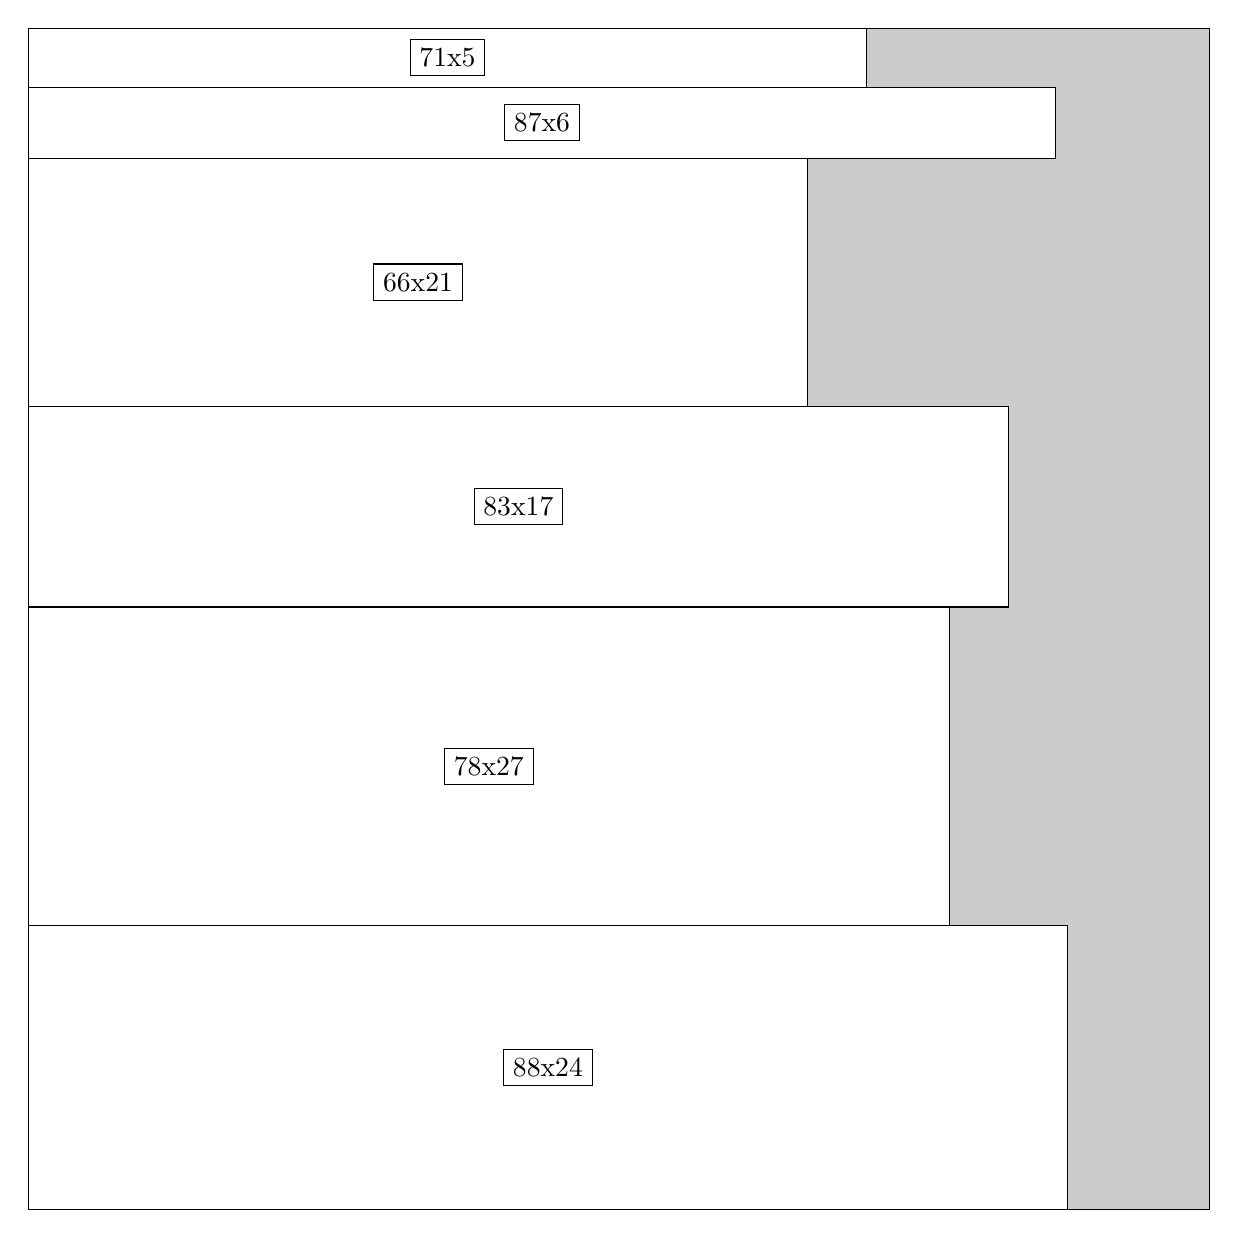
\begin{tikzpicture}[shorten >=1pt,scale=1.0,every node/.style={scale=1.0},->]
\tikzstyle{vertex}=[circle,fill=black!25,minimum size=14pt,inner sep=0pt]
\filldraw[fill=gray!40!white, draw=black] (0,0) rectangle (15.0,15.0);
\foreach \name/\x/\y/\w/\h in {88x24/0.0/0.0/13.2/3.5999999999999996,78x27/0.0/3.5999999999999996/11.7/4.05,83x17/0.0/7.6499999999999995/12.45/2.55,66x21/0.0/10.2/9.9/3.15,87x6/0.0/13.35/13.049999999999999/0.8999999999999999,71x5/0.0/14.25/10.65/0.75}
\filldraw[fill=white!40!white, draw=black] (\x,\y) rectangle node[draw] (\name) {\name} ++(\w,\h);
\end{tikzpicture}


w =88 , h =24 , x =0 , y =0 , v =2112
\par
w =78 , h =27 , x =0 , y =24 , v =2106
\par
w =83 , h =17 , x =0 , y =51 , v =1411
\par
w =66 , h =21 , x =0 , y =68 , v =1386
\par
w =87 , h =6 , x =0 , y =89 , v =522
\par
w =71 , h =5 , x =0 , y =95 , v =355
\par
\newpage


\end{document}